\documentclass[8pt, aspectratio=169]{beamer}
\usetheme{Frankfurt}
\usecolortheme{beaver}

\usepackage[spanish]{babel}
\usepackage{amsmath}
\usepackage{amsfonts}
\usepackage{amssymb}
\usepackage{color}
\usepackage{xcolor}
\usepackage{listings}
\usepackage{graphicx}
\usepackage{wrapfig}

\definecolor{codegreen}{rgb}{0,0.6,0}
\definecolor{codegray}{rgb}{0.5,0.5,0.5}
\definecolor{codepurple}{rgb}{0.58,0,0.82}
\definecolor{backcolour}{rgb}{0.95,0.95,0.92}

\lstdefinestyle{mystyle}{
    commentstyle=\color{codegreen},
    keywordstyle=\color{magenta},
    numberstyle=\tiny\color{codegray},
    stringstyle=\color{codepurple},
    basicstyle=\ttfamily\footnotesize,
    breakatwhitespace=false,         
    breaklines=true,                 
    captionpos=b,                    
    keepspaces=true,                 
    numbers=left,                    
    numbersep=5pt,                  
    showspaces=false,                
    showstringspaces=false,
    showtabs=false,                  
    tabsize=2,
	xleftmargin=8pt
}

\lstset{style=mystyle, basicstyle=\scriptsize}

\author{Shao Jie Hu Chen \and Mario Megías Mateo \and Jesús Samuel García Carballo}
\title{Práctica 1. Análisis de Eficiencia de Algoritmos}
\subtitle{Algorítmica}
%\logo{
\includegraphics[scale=0.05]{logo-ugr.jpeg}}
\institute{Equipo Rojo}
%\date{}
%\subject{}
%\setbeamercovered{transparent}
\setbeamertemplate{navigation symbols}{}

\begin{document}
	
	\begin{frame}[plain]
		\maketitle
		% \begin{center}
		% 	
\includegraphics[scale=0.15]{logo-ugr.jpeg}
		% \end{center}
	\end{frame}
	
	\begin{frame}
		\frametitle{Índice de contenidos}
		\tableofcontents
	\end{frame}





	\section{Introducción}

	\begin{frame}
		\frametitle{Objetivos}

            Los objetivos de esta práctica son los siguientes:
            \begin{itemize}
                \item \textbf{Estudio teórico, empírico e híbrido} y \textbf{comparación} de los algoritmos de ordenación más empleados, verificando los resultados teóricos.
                \item \textbf{Estudio teórico, empírico e híbrido} de algoritmos de alta complejidad, poniendo especial énfasis en su \textbf{viabilidad} en diferentes equipos. 
                \item Estudio del \textbf{aumento de eficiencia} de un mismo algoritmo para diferentes \textbf{tipos de optimización} del compilador. 
                \item Determinación del algoritmo \textbf{más adecuado} para cada situación en función del estado de los datos.
            \end{itemize}

	\end{frame}

	\begin{frame}

        \frametitle{Equipo}

        \begin{block}{ASUS}
			\begin{itemize}
				\item \textbf{Modelo}: ZenBook 15 UX534F
				\item \textbf{Procesador}: Intel(R) Core(TM) i7-10510U CPU @ 1.80GHz5
				\item \textbf{Memoria Ram}: 16 GB DDR4 @ 2.133 MHz.
				\item \textbf{Sistema Operativo} Ubuntu 20.04.2 LTS
			\end{itemize}
		\end{block}
            
        \begin{block}{HP}
            \begin{itemize}
				\item \textbf{Modelo}: Pavilion Gaming Laptop 15-dk0xxx
				\item \textbf{Procesador}: Intel(R) Core(TM) i7-9750H CPU @ 2.60GHz
				\item \textbf{Memoria RAM:} 32 GB DDR4
				\item \textbf{Sistema Operativo}: Ubuntu 20.04.4 LTS
			\end{itemize}
        \end{block}

        \begin{block}{LENOVO}
            \begin{itemize}
				\item \textbf{Modelo}: YOGA 530-14IKB
				\item \textbf{Procesador}: Intel(R) Core(TM) i5-8250U CPU @ 1.60GHz
				\item \textbf{Memoria RAM:} 8 GB DDR4
				\item \textbf{Sistema Operativo}: Ubuntu 20.04.4 LTS
			\end{itemize}
        \end{block}
    \end{frame}

    \begin{frame}
        \frametitle{Metodología}    
        \begin{figure}[H]
			\centering
			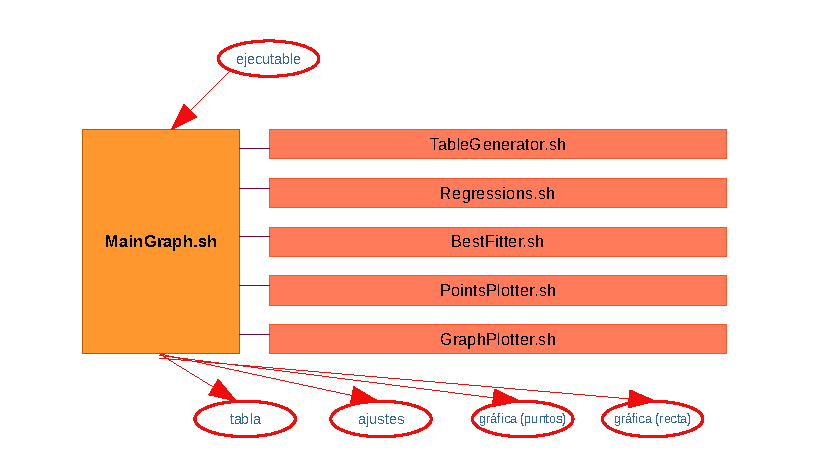
\includegraphics[width=0.67\textwidth]{img/esquema_graphkiller.pdf}
			\caption{Esquema del funcionamiento de GraphKiller}
			\label{graph-killer}
		\end{figure}
    \end{frame}




    \section{Análisis de Eficiencia General}

    \begin{frame}
        \frametitle{Eficiencia teórica}
        
        % \begin{itemize}
        %     \item \textbf{HeapSort}: $O(nlog(n))$
        %     \item  \textbf{QuickSort}: $T(n) \in O(nlog_{2}(n))$ si n $\geq$ UMBRAL.
        %     \item  \textbf{Inserción}: 
        %     \item  \textbf{Selección}:
        %     \item  \textbf{Heaport}:
        %     \item  \textbf{Heaport}:
        %     \item  \textbf{Heaport}:
        % \end{itemize}

        % \begin{columns}
		% 	% Column 1
		% 	\begin{column}{0.5\textwidth}
		% 		\begin{exampleblock}{Ejemplo de código}
        %             \lstinputlisting[language=C++, firstline=56, lastline=68]{../src/heapsort.cpp} 
        %         \end{exampleblock}
		% 	\end{column}
		% 	% Column 2    
		% 	\begin{column}{0.5\textwidth}

		% 		\begin{exampleblock}{Ejemplo de código}
        %             \lstinputlisting[language=C++, firstline=56, lastline=68]{../src/heapsort.cpp} 
        %         \end{exampleblock}

				

		% 	\end{column}
		% 	\end{columns}

        \begin{columns}
            \begin{column}{0.4\textwidth}
                \begin{block}{Algoritmo HeapSort}
                    $$T(n) \in \mathcal{O}(n\cdot\log(n))$$
                \end{block}
            \end{column}

            \begin{column}{0.4\textwidth}
                \begin{alertblock}{Algoritmo QuickSort}
                    $$T(n) \in \mathcal{O}(n\cdot\log(n))$$
                \end{alertblock}
            \end{column}
        \end{columns}

        \begin{columns}
            \begin{column}{0.4\textwidth}
                \begin{alertblock}{Algoritmo de Inserción}
                    $$T(n) \in \mathcal{O}(n^2)$$
                \end{alertblock}
            \end{column}
            
            \begin{column}{0.4\textwidth}
                \begin{block}{Algoritmo de Selección}
                    $$T(n) \in \mathcal{O}(n^2)$$
                \end{block}
            \end{column}
        \end{columns}
        
        \begin{columns}
            \begin{column}{0.4\textwidth}
                \begin{alertblock}{Algoritmo de Floyd}
                    $$T(n) \in \mathcal{O}(n^3)$$
                \end{alertblock}
            \end{column}

            \begin{column}{0.4\textwidth}
                \begin{alertblock}{Algoritmo de Hanoi}
                    $$T(n) \in \mathcal{O}(2^n)$$
                \end{alertblock}
            \end{column}
        \end{columns}
        
        \vspace{1cm}
        Más \textbf{detalles} en la memoria de la práctica. 
    \end{frame}

    \begin{frame}
        \frametitle{Eficiencia empírica: Caso $T(n) \in \mathcal{O}(n\cdot\log(n))$}

        \begin{figure}
            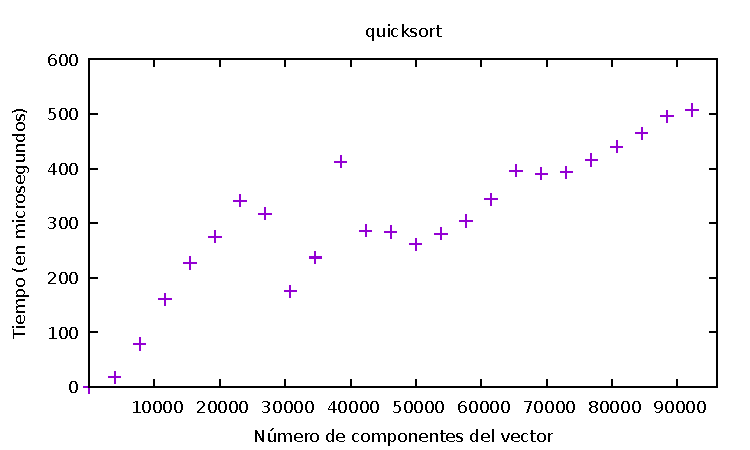
\includegraphics[width=0.7\textwidth]{../data/hp/quicksort-points.pdf}
            \caption{Gráfica de tiempos de ejecución (en $\mu$s) puntos del algoritmo QuickSort (HP)}
        \end{figure}
    \end{frame}

    \begin{frame}
        \frametitle{Eficiencia empírica: Caso $T(n) \in \mathcal{O}(n^2)$}

        \begin{figure}
            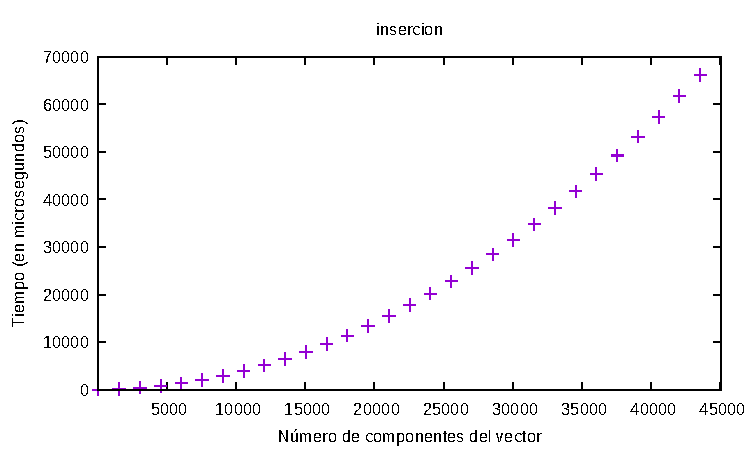
\includegraphics[width=0.7\textwidth]{../data/lenovo/insercion-points.pdf}
            \caption{Gráfica de tiempos de ejecución (en $\mu$s) puntos del algoritmo de Inserción (Lenovo)}
        \end{figure}
    \end{frame}

    \begin{frame}
        \frametitle{Eficiencia empírica: Caso $T(n) \in \mathcal{O}(n^3)$}

        \begin{columns}
            \begin{column}{0.5\textwidth}
                \begin{figure}
                    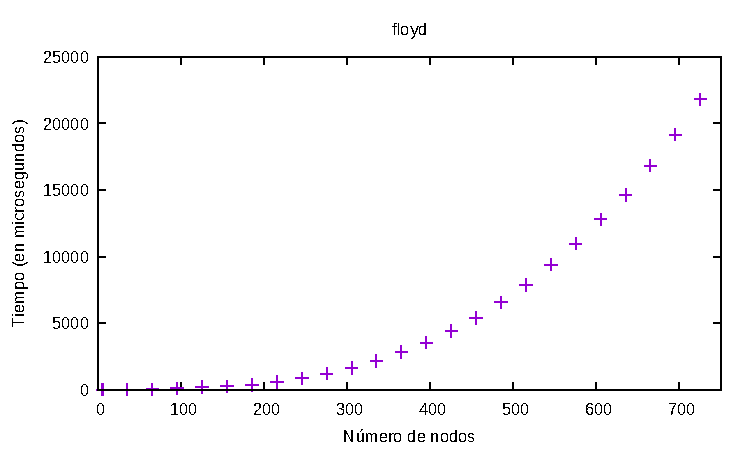
\includegraphics[width=0.85\textwidth]{../data/asus/floyd-points.pdf}
                    \caption{Gráfica de tiempos de ejecución (en $\mu$s) puntos del algoritmo de Floyd (ASUS)}
                \end{figure}
            \end{column}
            \begin{column}{0.5\textwidth}
                \begin{figure}
                    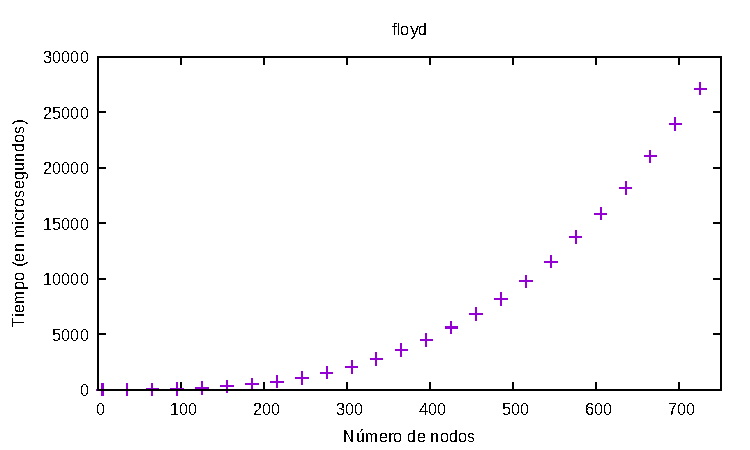
\includegraphics[width=0.85\textwidth]{../data/lenovo/floyd-points.pdf}
                    \caption{Gráfica de tiempos de ejecución (en $\mu$s) puntos del algoritmo de Floyd (Lenovo)}
                \end{figure}
            \end{column}
        \end{columns}

        
    \end{frame}

    \begin{frame}
        \frametitle{Eficiencia empírica: Caso $T(n) \in \mathcal{O}(2^n)$}

        \begin{figure}
            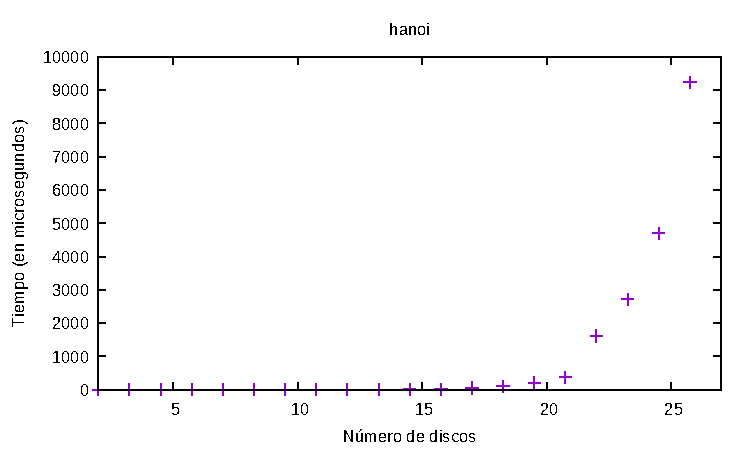
\includegraphics[width=0.87\textwidth]{../data/lenovo/hanoi-points.pdf}
            \caption{Gráfica de tiempos de ejecución (en $\mu$s) puntos del algoritmo de Hanoi (Lenovo)}
        \end{figure}
        
    \end{frame}

    \begin{frame}
        \frametitle{Eficiencia híbrida: Algoritmo QuickSort}

        \begin{columns}
            \begin{column}{0.7\textwidth}
                \begin{figure}
                    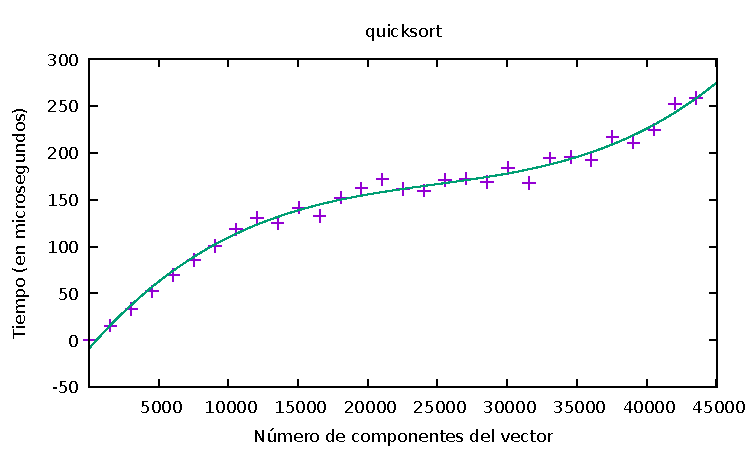
\includegraphics[width=0.65\textwidth]{../data/hp/quicksort-graph.pdf}
                    \caption{Gráfica de tiempos de ejecución (en $\mu$s) puntos del algoritmo de Inserción (HP) con función de ajuste}
                \end{figure}
            \end{column}

            \begin{column}{0.3\textwidth}
                \begin{block}{Función de ajuste}
                    $f(x) = 3.66 \cdot 10^{-4} x \log(x) + 50$
                \end{block}

                \begin{block}{Coeficiente de determinación}
                    $R^2 = 0.9957$
                \end{block}
            \end{column}
        \end{columns}
    \end{frame}

    \begin{frame}
        \frametitle{Eficiencia híbrida: Algoritmo Inserción}

        \begin{columns}
            \begin{column}{0.7\textwidth}
                \begin{figure}
                    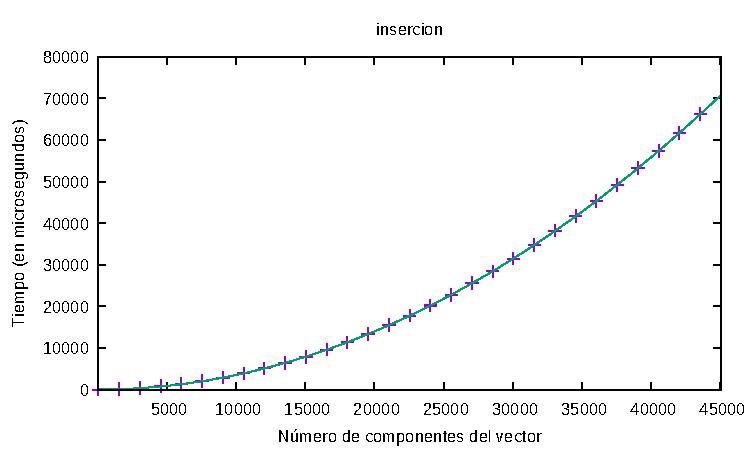
\includegraphics[width=0.65\textwidth]{../data/lenovo/insercion-graph.pdf}
                    \caption{Gráfica de tiempos de ejecución (en $\mu$s) puntos del algoritmo de Inserción (Lenovo) con función de ajuste}
                \end{figure}
            \end{column}

            \begin{column}{0.3\textwidth}
                \begin{block}{Función de ajuste}
                    $f(x) =3.48955 \cdot 10^{-5} x^{2} - 0.000620098 x + 48.0855$
                \end{block}

                \begin{block}{Coeficiente de determinación}
                    $R^2 = 0.99999$
                \end{block}
            \end{column}
        \end{columns}
    \end{frame}

    \begin{frame}
        \frametitle{Eficiencia híbrida: Algoritmo Floyd}

        \begin{columns}
            \begin{column}{0.7\textwidth}
                \begin{figure}
                    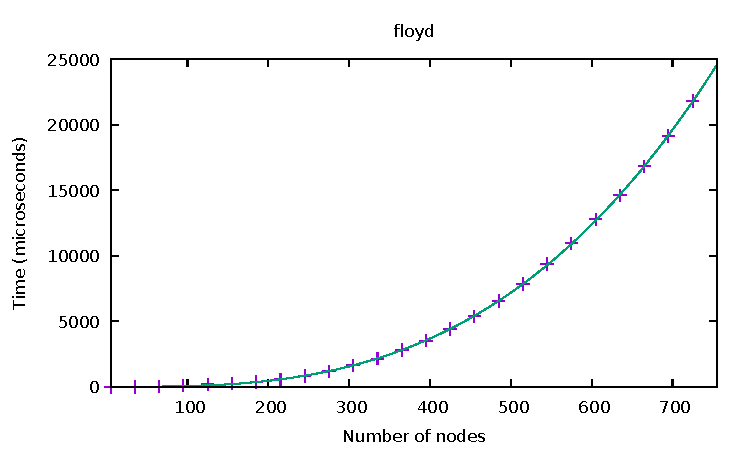
\includegraphics[width=0.65\textwidth]{../data/asus/floyd-graph.pdf}
                    \caption{Gráfica de tiempos de ejecución (en $\mu$s) puntos del algoritmo de Floyd (Asus) con función de ajuste}
                \end{figure}
            \end{column}

            \begin{column}{0.3\textwidth}
                \begin{block}{Función de ajuste}
                    $f(x) = 5.57676 \cdot 10^{-5} x^3 + 0.00138722 x^2-0.315202 x + 34.0467$
                \end{block}

                \begin{block}{Coeficiente de determinación}
                    $R^2 = 1.0000$
                \end{block}
            \end{column}
        \end{columns}
    \end{frame}

    \begin{frame}
        \frametitle{Eficiencia híbrida: Algoritmo Hanoi}

        \begin{columns}
            \begin{column}{0.7\textwidth}
                \begin{figure}
                    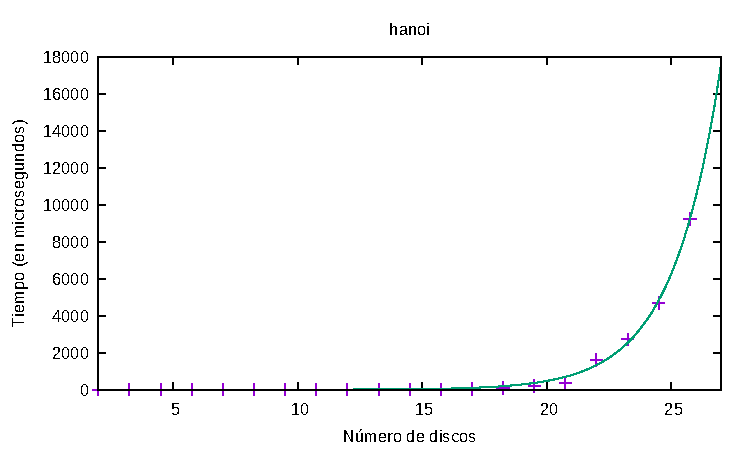
\includegraphics[width=0.65\textwidth]{../data/lenovo/hanoi-graph.pdf}
                    \caption{Gráfica de tiempos de ejecución (en $\mu$s) puntos del algoritmo de Hanoi (Lenovo) con función de ajuste}
                \end{figure}
            \end{column}

            \begin{column}{0.3\textwidth}
                \begin{block}{Función de ajuste}
                    $f(x) = 0.0158 \cdot e^{0.503814 x}$
                \end{block}

                \begin{block}{Coeficiente de determinación}
                    $R^2 = 0.9921$
                \end{block}
            \end{column}
        \end{columns}
    \end{frame}

    \section{Análisis de Casos Particulares}

    \begin{frame}
        \frametitle{Niveles de Optimización}

        \begin{columns}
            \begin{column}{0.7\textwidth} 
                \begin{figure}
                    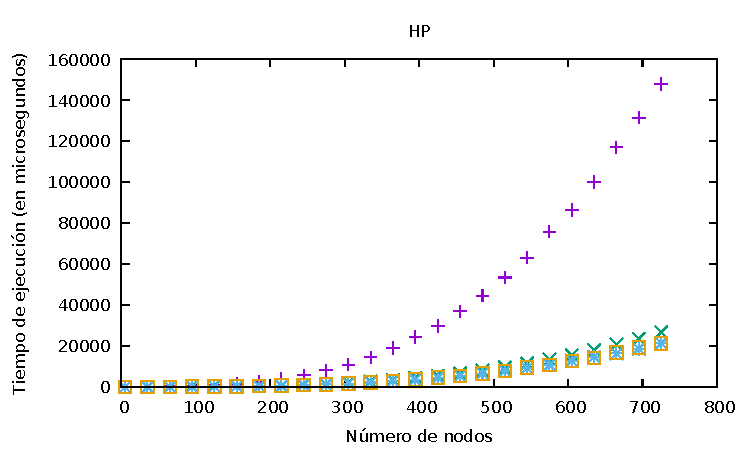
\includegraphics[width=0.65\textwidth]{../data/hp_opt.pdf}
                    \caption{Gráfica de tiempos de ejecución (HP) en diferentes niveles de optimización}
                \end{figure}
            \end{column}

            \begin{column}{0.3\textwidth}
                \begin{itemize}
                    \item \textcolor{purple}{Morado}: O0
                    \item \textcolor{green}{Verde}: O1
                    \item \textcolor{yellow}{Amarillo}: O2
                    \item \textcolor{blue}{Azul}: O3 
                \end{itemize}
            \end{column}
        \end{columns}
        
    \end{frame}

    \begin{frame}
        \frametitle{Comparación de algoritmos de ordenación}

        \begin{figure}
            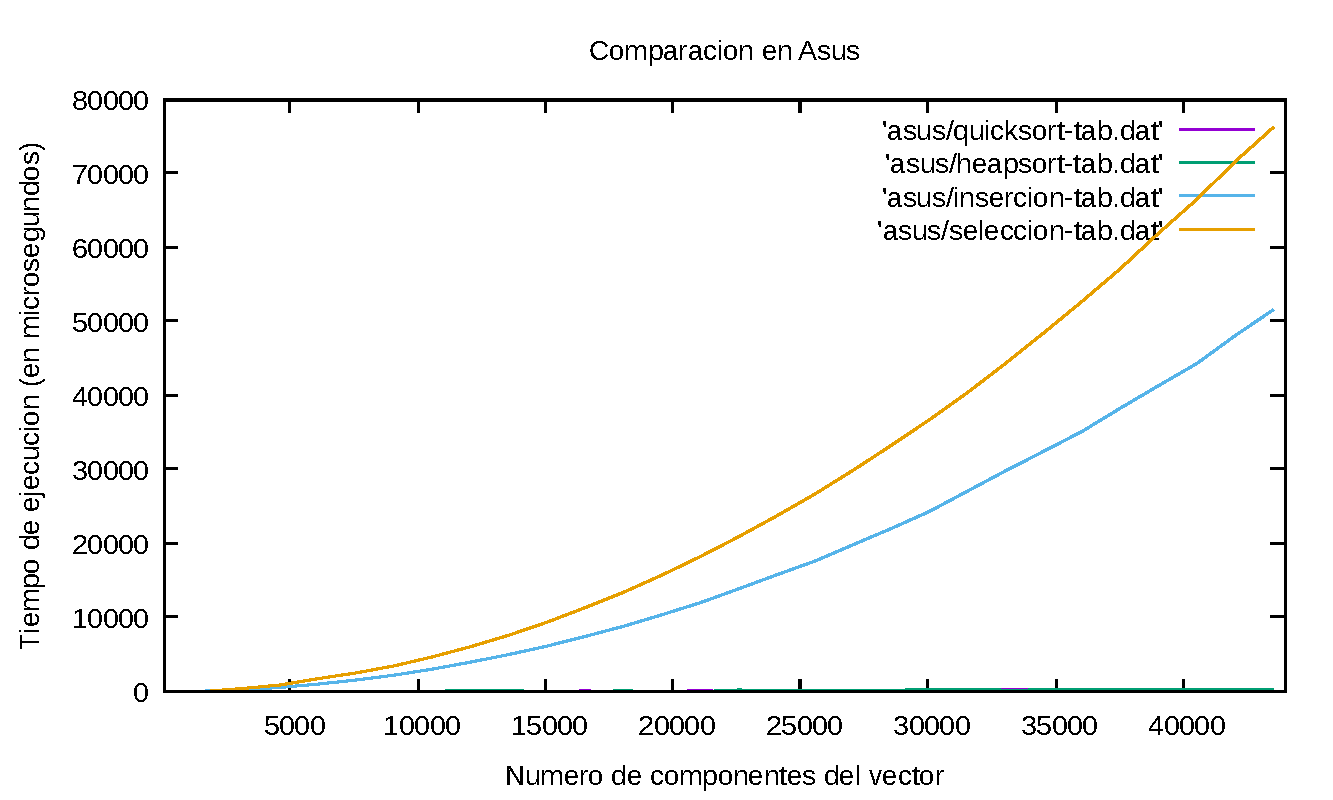
\includegraphics[width=0.8\textwidth]{../data/asus-orden-todos.pdf}
            \caption{Gráfica de tiempos de ejecución (ASUS) para diferentes algoritmos de ordenación}
        \end{figure}
    \end{frame}

    \begin{frame}
        \frametitle{Mejor y peor caso para Inserción}

        \begin{figure}
            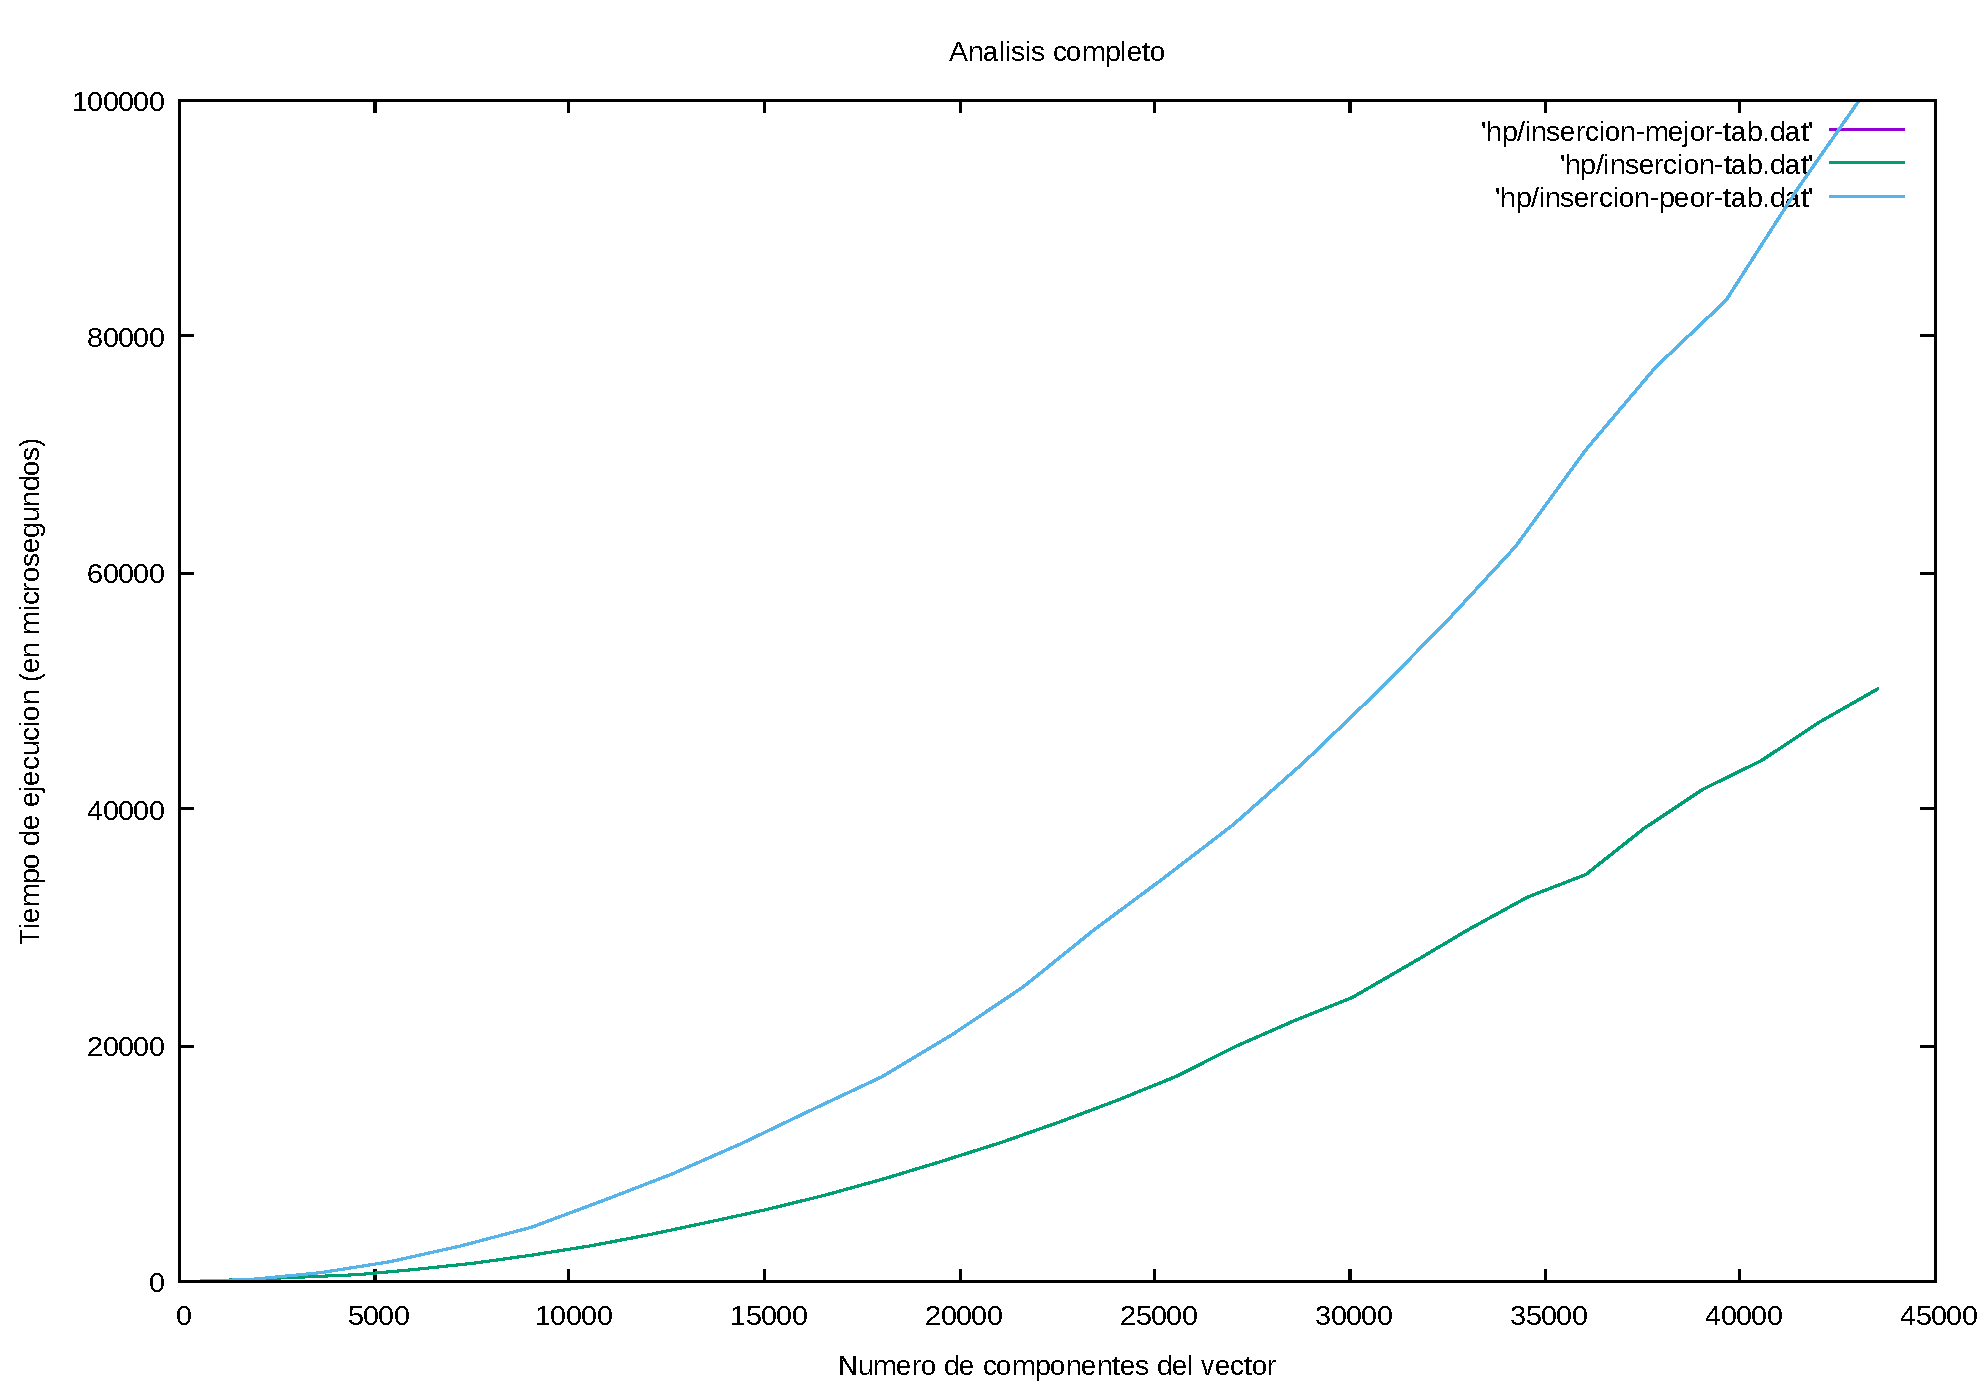
\includegraphics[width=0.7\textwidth]{../data/hp-insercion-mp.pdf}
            \caption{Gráfica de tiempos de ejecución (HP) para Inserción}
        \end{figure}
    \end{frame}

    \begin{frame}
        \frametitle{Mejor y Peor Caso para Selección}
        \begin{figure}
            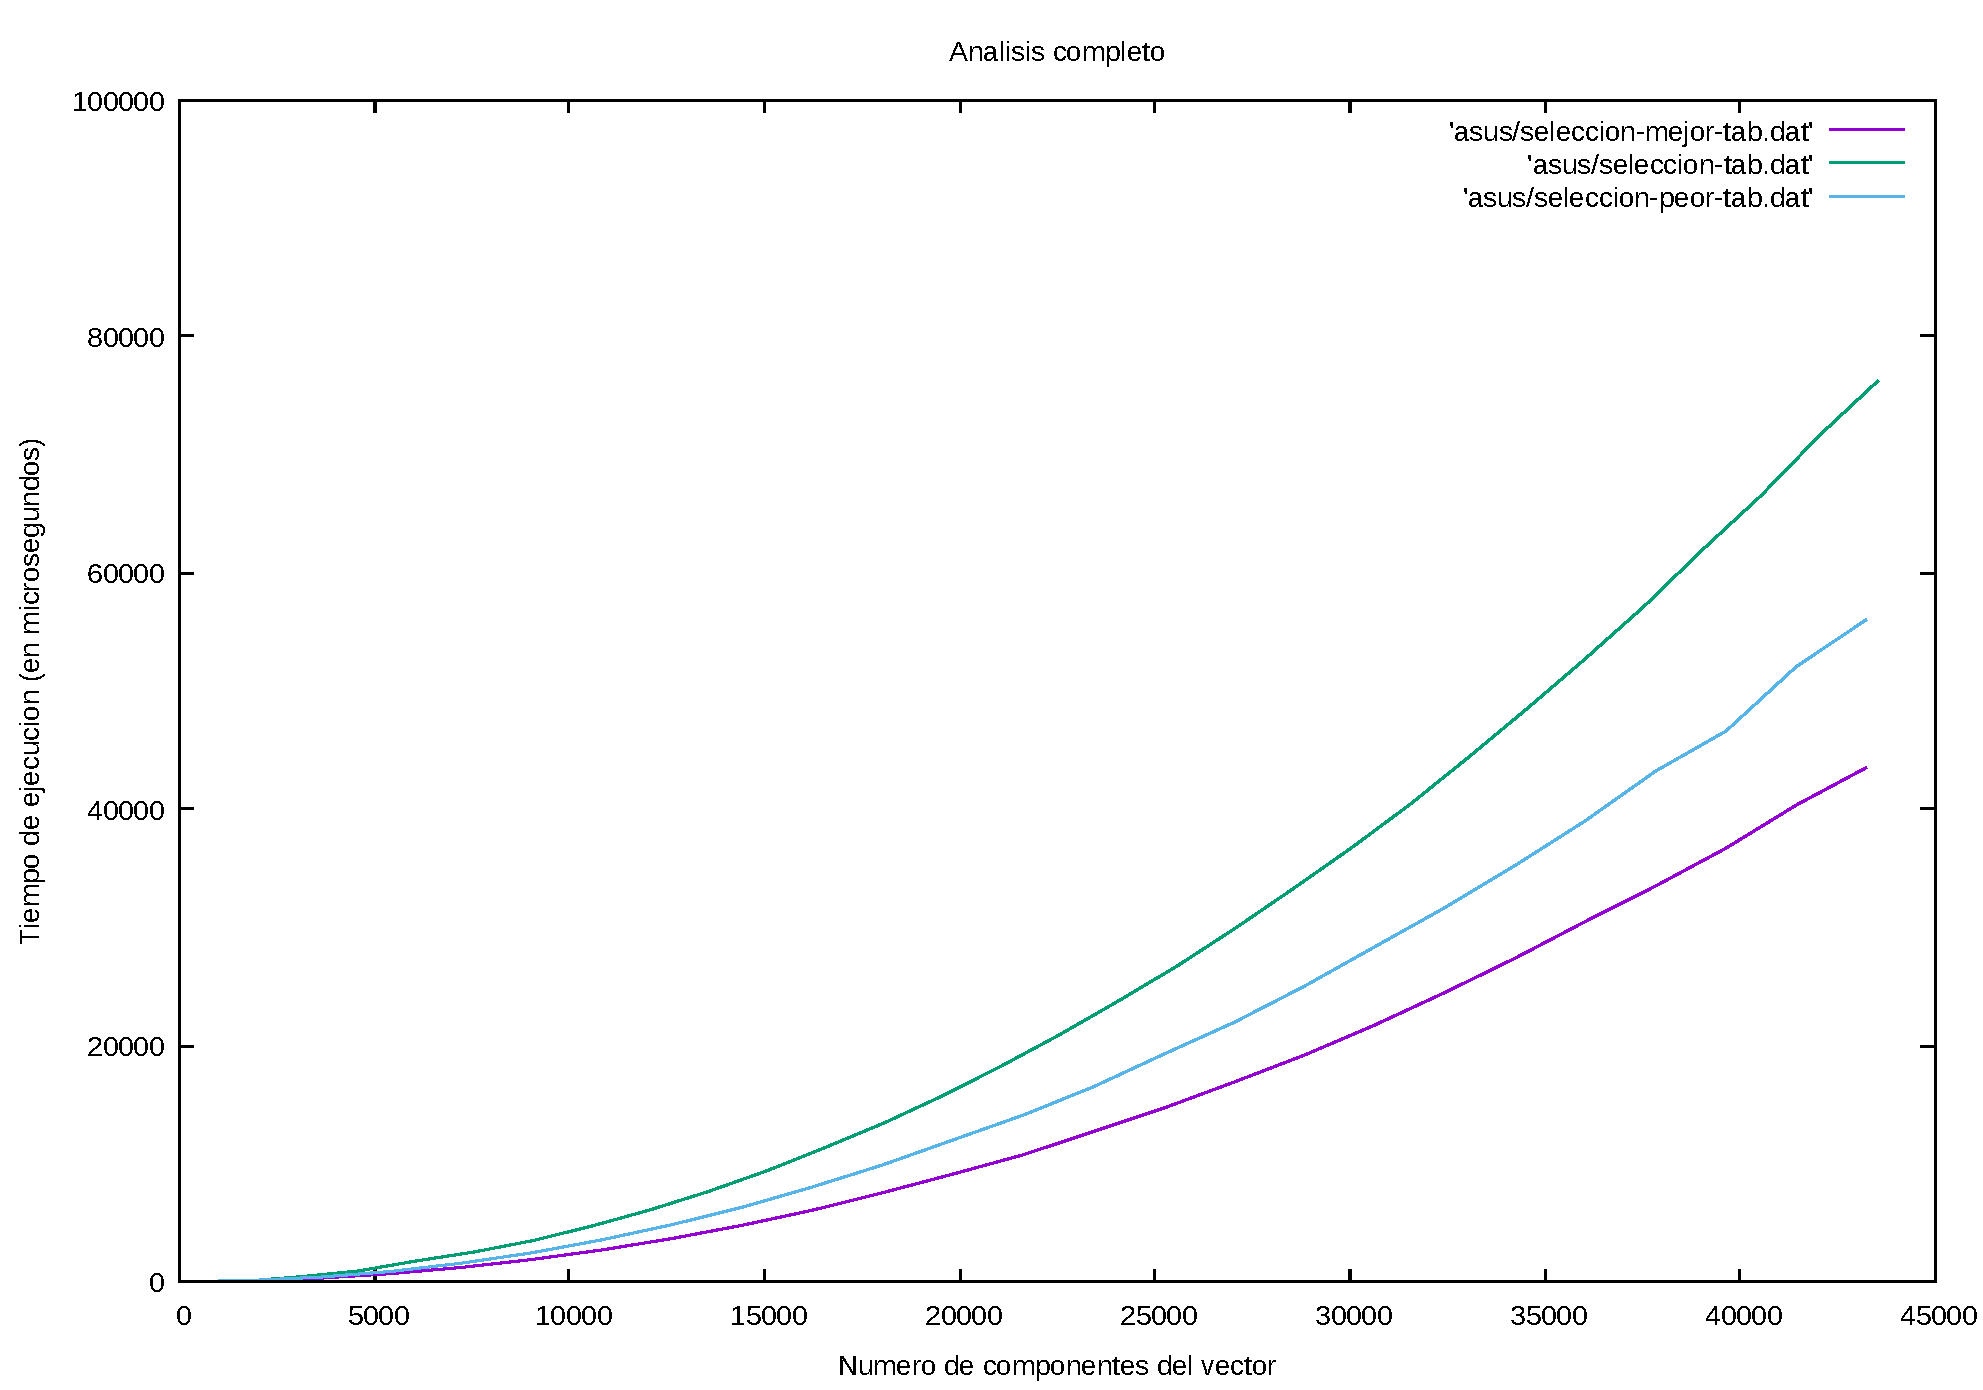
\includegraphics[width=0.7\textwidth]{../data/asus-seleccion-mp.pdf}
            \caption{Gráfica de tiempos de ejecución (ASUS) para Selección}
        \end{figure}
    \end{frame}

    \section{Conclusiones}

    \begin{frame}
        \frametitle{Conclusiones}

        Los aspectos tratados más relevantes son:

        \begin{itemize}
            \item \textbf{Comprobar que los análisis empíricos verifican los resultados teóricos esperados}.
            Calculado los coeficientes de determinación comprobamos que la función de regresión que mejor se 
            ajusta en cada caso coincide con el tipo de función dado por el análisis teórico.
            \item \textbf{Comparar los resultados experimentales en equipos distintos}. Hemos ilustrado que los 
            tiempos de ejecución de un mismo algortimo se reducen con un mejor hardware.
            \item \textbf{Cómo elegir un algoritmo de ordenación}. Para grandes tamaños de problema conviene escoger
            los de mejor orden de eficiencia mientras que para tamaños inferiores es indiferente.
            \item \textbf{Análisis del peor y mejor caso en Selección e Inserción}. El tiempo de ejecución se reduce considerablemente
            en vectores ordenados ascendentemente, y aumenta en vectores ordenados descendentemente, sobre todo en Inserción. 
            \item \textbf{Comparar los tiempos de ejecución para optimizaciones distintas}. Para tamaños pequeños
            las diferencias no son apreciables, en cambio para valores mayores estas se acentúan.
        \end{itemize}
        
    \end{frame}

    \section{Referencias}

    \begin{frame}
        \begin{thebibliography}{0}
            \bibitem{Verdegay2017} Verdegay Galdeano. (2017). Lecciones de Algorítmica / José Luis Verdegay. Técnica Avicam.
            \bibitem{Cormen2017} Cormen. (2017). Introduction to algorithms / Thomas H. Cormen... [et al.] (3rd ed.). PHI Learning.
            \bibitem{Garrido2018} Garrido Carrillo. (2018). Estructuras de datos avanzadas: con soluciones en C++ / A. Garrido. Universidad de Granada.        
        \end{thebibliography}
    \end{frame}
    

	
\end{document}